\documentclass[11pt,a4paper]{article}

% ── Self-contained preamble (mirrors FSA_version_5_technical_guide.tex) ─────
\usepackage[utf8]{inputenc}
\usepackage[T1]{fontenc}
\usepackage{lmodern}
\usepackage{amsmath, amssymb, amsthm}
\usepackage{graphicx}
\usepackage{booktabs}
\usepackage{longtable}
\usepackage{hyperref}
\usepackage{url}
\usepackage{geometry}
\usepackage{xcolor}
\usepackage{listings}
\usepackage{bm}

\geometry{margin=1in}

\hypersetup{
    colorlinks=true,
    linkcolor=blue,
    filecolor=magenta,
    urlcolor=cyan,
}

\newtheorem{theorem}{Theorem}
\newtheorem{lemma}[theorem]{Lemma}
\newtheorem{proposition}[theorem]{Proposition}
\newtheorem{corollary}[theorem]{Corollary}
\theoremstyle{definition}
\newtheorem{definition}[theorem]{Definition}
\newtheorem{remark}[theorem]{Remark}

\newcommand{\R}{\mathbb{R}}
\newcommand{\dd}{\,\mathrm{d}}

\lstset{
  basicstyle=\ttfamily\small,
  breaklines=true,
  showstringspaces=false,
  frame=single,
  framerule=0.3pt,
  rulecolor=\color{gray!50},
  xleftmargin=0.5em,
  xrightmargin=0.5em,
  aboveskip=0.6em,
  belowskip=0.6em,
  extendedchars=true,
  inputencoding=utf8,
  literate=
    {μ}{{$\mu$}}1
    {Φ}{{$\Phi$}}1
    {κ}{{$\kappa$}}1
    {τ}{{$\tau$}}1
    {η}{{$\eta$}}1
    {ℝ}{{$\mathbb{R}$}}1
    {ε}{{$\varepsilon$}}1
    {λ}{{$\lambda$}}1
    {α}{{$\alpha$}}1
    {β}{{$\beta$}}1
    {δ}{{$\delta$}}1
    {≥}{{$\geq$}}1
    {≤}{{$\leq$}}1
    {≈}{{$\approx$}}1
    {→}{{$\to$}}1
    {↔}{{$\leftrightarrow$}}1
    {±}{{$\pm$}}1
    {·}{{$\cdot$}}1
    {×}{{$\times$}}1
    {²}{{$^2$}}1
    {³}{{$^3$}}1
    {₀}{{$_0$}}1
    {₁}{{$_1$}}1
    {₂}{{$_2$}}1
    {ν}{{$\nu$}}1
    {θ}{{$\theta$}}1
    {Δ}{{$\Delta$}}1
    {√}{{$\sqrt{}$}}1
    {∀}{{$\forall$}}1
    {∈}{{$\in$}}1
    {–}{{--}}1
    {—}{{---}}1
    {ö}{{\"o}}1
}

\title{FSA-v5 Controllability: Four Constructive Proofs\\
\large under the v2 re-parametrisation, ready for Lean4 mechanisation}
\author{Claude (Anthropic) under direction of Ajay Talati}
\date{2026-05-11}

\begin{document}

\maketitle

\begin{abstract}
We present four constructive controllability theorems for the deterministic FSA-v5 dynamics under a revised parametrisation \texttt{RECOMMENDED\_V2} that shifts the healthy attractor from $\Phi \approx (0.30, 0.30)$ to $\Phi \approx (1.06, 0.78)$ and widens the basin of attraction substantially. Each theorem exhibits a constant control witness $\Phi^* \in \R_{\ge 0}^2$ and verifies the qualitative outcome by direct RK4 integration of the 6-D ODE: (1) the sedentary basin is still pathological — $\Phi \equiv (0.1, 0.1)$ from \texttt{SEDENTARY\_INIT} drives $A \to 0$; (2) constructive escape — the FIM-duality-selected witness $\Phi^* = (0.86, 1.24)$ takes $A$ from $0.10$ to $1.16$ in $T = 100$\,d; (3) the over-training basin still exists (shifted to higher $\Phi$) — $\Phi \equiv (2.5, 2.5)$ from the v2-redefined trained state drives $A \to 0$; (4) constructive maintenance — $\Phi \equiv (1, 1)$ holds the trained state at $A^* = 1.238$. Witness selection for (2) uses the Fisher Information Matrix of the trajectory with $\Phi$ as the parameter to identify, exploiting the classical identification $\leftrightarrow$ controllability duality.

\medskip\noindent\textbf{Scope statement 1: v2 is a re-parametrisation, not a re-modelling.} The mathematical structure of FSA-v5 (state, drift, observation model, slow-manifold cascade) is unchanged. Only the numerical values of 8 parameters differ from canonical \texttt{TRUTH\_PARAMS\_V5}. The existing \texttt{Fsa.V5.*} Lean specifications and Julia dynamics modules need no structural edits. Numerical verification is fully self-contained in Appendix~2.2's standalone Julia script (no project dependencies). The only code-change prerequisite to run the SMC$^2$-MPC bench under v2 is a small CLI-flag addition ($<$100 LOC); see §\ref{sec:todo}.

\medskip\noindent\textbf{Scope statement 2: FIM identifiability under v2 is open.} The existing tech-guide §15 Fisher-information analysis was performed under canonical parameters. v2 alters dynamics timescales, fatigue penalties, and deconditioning thresholds by factors of 2 to 10, all of which substantially change the FIM structure. A repeat identifiability analysis under v2 is a prerequisite for production deployment but is out of scope here; see §\ref{sec:todo}.

\medskip\noindent\textbf{Companion document}: the longer investigative writeup \texttt{sedentary\_basin\_controllability.tex} in this directory contains the impossibility analysis under canonical parameters, the multi-parameter sweep that produced the v2 recommendation, and intermediate witness-design attempts. The present document is its streamlined LEAN-ready successor; the investigative material is not a dependency.
\end{abstract}

\tableofcontents

\bigskip

% =============================================================================
\section{Introduction} \label{sec:intro}
% =============================================================================

\subsection{What this document is}

This document presents four constructive controllability theorems for the deterministic FSA-v5 dynamics. ``Constructive'' here means: each theorem identifies an explicit constant control $\Phi^* \in \R_{\ge 0}^2$ as the witness, and the proof obligation reduces to a finite ODE integration with an end-time inequality check.

The four theorems together describe the qualitative phase portrait of the model under v2 parameters from two physiologically meaningful initial conditions (sedentary, trained-athlete):

\begin{itemize}
  \item from \texttt{SEDENTARY\_INIT}, passive low-effort policy drives autonomic collapse (Theorem~\ref{thm:t61}); a specific moderate-effort constant policy escapes the basin to the healthy attractor (Theorem~\ref{thm:t62});
  \item from \texttt{TRAINED\_ATHLETE\_INIT\_v2}, passive heavy over-load policy drives autonomic collapse (Theorem~\ref{thm:t63}); the natural maintenance policy at the island centre holds the trained equilibrium (Theorem~\ref{thm:t64}).
\end{itemize}

The witness for Theorem~\ref{thm:t62} is selected by an identification-$\leftrightarrow$-controllability duality argument: among all constant $\Phi$, the one that minimises the condition number of the trajectory Fisher Information Matrix (with $\Phi$ treated as the parameter to identify) is also a $\Phi$ where both control axes have strong effect on the state — i.e., a controllable witness. Section~\ref{sec:fim-witness} develops this.

\subsection{Working assumptions}

\begin{enumerate}
  \item \textbf{Deterministic dynamics.} We work with the deterministic ODE underlying the FSA-v5 SDE; stochastic extension is out of scope.
  \item \textbf{Full observability.} The control law has access to the 6-D state $y = (B, S, F, A, K_{FB}, K_{FS})$ exactly. The closed-loop SMC$^2$-MPC bench's particle filter is removed from consideration.
  \item \textbf{Canonical mathematical structure.} All state variables, drift equations, slow-manifold cascade relations, and observation channels are identical to canonical FSA-v5 (per the tech guide). Only parameter values change.
  \item \textbf{Single admissible control set.} $\Phi(t) \in \R_{\ge 0}^2$. We do not impose an upper bound such as $\Phi_{\max} = 3$; the witnesses below have $\Phi^* \in [0.1, 2.5]^2$ and lie comfortably inside any reasonable bound.
\end{enumerate}

\subsection{Why this document exists}

A T=100-d closed-loop SMC$^2$-MPC bench (2026-05-11) under canonical FSA-v5 parameters failed to escape the sedentary basin from \texttt{SEDENTARY\_INIT}: $A$ decayed from $0.10$ to $0.003$ despite a heavily upgraded controller. The companion investigative document argued, with strong numerical evidence, that this failure is structural — the canonical parametrisation has a healthy attractor at $\Phi \approx (0.30, 0.30)$ that is unreachable from \texttt{SEDENTARY\_INIT} in $T = 100$\,d under any admissible $\Phi$. The companion document then explored model modifications and proposed the v2 parametrisation specified in §\ref{sec:model-recall} below, under which the four theorems of §\ref{sec:theorems} hold. The bench failure was therefore a model issue, not a controller-tuning issue.

\subsection{Document outline}

§\ref{sec:model-recall} gives a self-contained model recall under v2. §\ref{sec:control} defines the controllability target. §\ref{sec:cascade} summarises the slow-manifold cascade structure. §\ref{sec:island-geometry} characterises the healthy-island geometry under v2. §\ref{sec:theorems} states and proves (constructively, by direct integration) the four theorems. §\ref{sec:fim-witness} explains the FIM-duality witness selection. §\ref{sec:closed-loop} discusses implications for closed-loop control. §\ref{sec:lean-roadmap} maps each theorem to its expected Lean4 mechanisation. §\ref{sec:todo} flags three open items: bench CLI exposure, v2 FIM identifiability, and SMC$^2$ cost-function tuning. Appendix~1 is the numerical-anchor table; Appendix~2 contains Lean4 theorem stubs and the standalone Julia reference script.

% =============================================================================
\section{Model recall under \texttt{RECOMMENDED\_V2}} \label{sec:model-recall}
% =============================================================================

This section is the canonical model reference. A verifier should be able to implement the dynamics directly from these equations and parameter tables.

\subsection{State and control}

The 6-D state $y \in \R^6$:
\[
y \;=\; (B,\; S,\; F,\; A,\; K_{FB},\; K_{FS})^\top.
\]

Component meanings, ranges, and typical values:
\begin{center}\small
\begin{tabular}{lllp{6.3cm}}
\toprule
Symbol & Range & Typical & Physical meaning \\
\midrule
$B$       & $[0, 1]$       & $0.5$ (trained), $0.05$ (sedentary)  & Chronic aerobic-fitness capacity. \\
$S$       & $[0, 1]$       & $0.45$ (trained), $0.10$ (sedentary) & Chronic strength capacity. \\
$F$       & $[0, \infty)$  & $0.20 = F_{\rm TYP}$ (rest), $0.8$ (mild load) & Unified short-term fatigue. \\
$A$       & $[0, \infty)$  & $1.24$ (trained-v2), $0.10$ (sedentary)   & Autonomic amplitude (HRV proxy). \\
$K_{FB}$  & $[0, \infty)$  & $0.030$ baseline                           & Aerobic fatigue-sensitivity gain. \\
$K_{FS}$  & $[0, \infty)$  & $0.050$ baseline                           & Strength fatigue-sensitivity gain. \\
\bottomrule
\end{tabular}
\end{center}

Control: $\Phi(t) = (\Phi_B(t), \Phi_S(t)) \in \R_{\ge 0}^2$.

\subsection{Drift equations}

Writing $a_X(A) = (1 + \epsilon_{AX} A)/(1 + \epsilon_{AX} A_{\rm TYP})$ for $X \in \{AB, AS\}$ and $a_F(A) = (1 + \lambda_A A)/(1 + \lambda_A A_{\rm TYP})$:

\begin{align}
\dot B   &= \kappa_B \, a_B(A) \, \Phi_B - B / \tau_B \label{eq:drift-B}\\
\dot S   &= \kappa_S \, a_S(A) \, \Phi_S - S / \tau_S \label{eq:drift-S}\\
\dot F   &= K_{FB} \Phi_B + K_{FS} \Phi_S - a_F(A) F / \tau_F \label{eq:drift-F}\\
\dot A   &= \mu(B, S, F) \, A - \eta A^3 \label{eq:drift-A}\\
\dot K_{Fi} &= (K_{Fi}^0 - K_{Fi}) / \tau_K + \mu_K \Phi_i, \quad i \in \{B, S\} \label{eq:drift-K}
\end{align}

The bifurcation parameter $\mu(B, S, F)$ governing autonomic dynamics is, in the v5 form with Hill deconditioning:
\begin{equation}
\boxed{\;
\mu(B, S, F) \;=\; \mu_0 + \mu_B B + \mu_S S - \mu_F F - \mu_{FF}(F - F_{\rm TYP})^2 - \mu_{B-} h_n(B; B_{\rm dec}) - \mu_{S-} h_n(S; S_{\rm dec})
\;}
\label{eq:mu}
\end{equation}
where the Hill saturation function
\begin{equation}
h_n(x; x_{\rm dec}) \;=\; \frac{x_{\rm dec}^n}{x^n + x_{\rm dec}^n} \;\in\; [0, 1]
\label{eq:hill}
\end{equation}
saturates to $1$ as $x \to 0$ (full deconditioning penalty) and drops to $0$ as $x \gg x_{\rm dec}$ (well-trained, no penalty).

\subsection{The \texttt{RECOMMENDED\_V2} parameter set}

Under v2, eight numerical parameters differ from canonical \texttt{TRUTH\_PARAMS\_V5}. All other parameters retain their canonical values.

\begin{center}\small
\begin{tabular}{llll}
\toprule
Parameter & Canonical value & v2 value & Notes \\
\midrule
\multicolumn{4}{l}{\emph{Time-scale halving (preserves slow-manifold equilibria)}} \\
$\tau_B$         & $42$\,d              & $\boldsymbol{21}$\,d                         & halved \\
$\kappa_B$       & $0.012(1 + 0.40 A_{\rm TYP}) = 0.01248$ & $\boldsymbol{0.02496}$    & doubled (centred form) \\
$\tau_S$         & $60$\,d              & $\boldsymbol{30}$\,d                         & halved \\
$\kappa_S$       & $0.008(1 + 0.20 A_{\rm TYP}) = 0.00816$ & $\boldsymbol{0.01632}$    & doubled (centred form) \\
\midrule
\multicolumn{4}{l}{\emph{Hill deconditioning threshold raised (shifts island toward $(1,1)$)}} \\
$B_{\rm dec}$    & $0.07$               & $\boldsymbol{0.25}$                          & raised $3.6\times$ \\
$S_{\rm dec}$    & $0.07$               & $\boldsymbol{0.25}$                          & raised $3.6\times$ \\
\midrule
\multicolumn{4}{l}{\emph{Reward-side fatigue penalty reduced (allows higher $\Phi$ to be healthy)}} \\
$\mu_F$          & $0.10 + 2 F_{\rm TYP} \cdot 0.40 = 0.26$ & $\boldsymbol{0.030}$        & reduced $88\%$ \\
$\mu_{FF}$       & $0.40$               & $\boldsymbol{0.020}$                         & reduced $95\%$ \\
\bottomrule
\end{tabular}
\end{center}

All other parameters are inherited from canonical \texttt{TRUTH\_PARAMS\_V5} unchanged:

\begin{center}\small
\begin{tabular}{lll lll}
\toprule
Parameter & Value & & Parameter & Value \\
\midrule
$A_{\rm TYP}$    & $0.10$ &  & $\mu_0$          & $0.02 + 0.40 \cdot F_{\rm TYP}^2 = 0.036$ \\
$F_{\rm TYP}$    & $0.20$ &  & $\mu_B$           & $0.30$ \\
$\epsilon_{AB}$  & $0.40$ &  & $\mu_S$           & $0.15$ \\
$\epsilon_{AS}$  & $0.20$ &  & $\mu_{B-}$       & $0.10$ \\
$\lambda_A$      & $1.00$ &  & $\mu_{S-}$       & $0.10$ \\
$\tau_F$         & $7.0/(1 + A_{\rm TYP}) = 6.36$\,d & & $n_{\rm dec}$ & $4$ \\
$K_{FB}^0$       & $0.030$ &  & $\eta$            & $0.20$ \\
$K_{FS}^0$       & $0.050$ &  & $\tau_K$         & $21$\,d \\
$\mu_K$          & $0.005$ &  & & \\
\bottomrule
\end{tabular}
\end{center}

\subsection{Initial conditions}

\paragraph{\texttt{SEDENTARY\_INIT}.} A deconditioned but not collapsed athlete:
\begin{equation}
\boxed{\;
\texttt{SEDENTARY\_INIT} \;=\; (B_0, S_0, F_0, A_0, K_{FB,0}, K_{FS,0}) \;=\; (0.05,\; 0.10,\; 0.30,\; 0.10,\; 0.030,\; 0.050).
\;}
\label{eq:sed-init}
\end{equation}
Note that under v2, $B_0 = 0.05$ is now \emph{well below} $B_{\rm dec} = 0.25$, so the Hill deconditioning term $h_4(B_0; B_{\rm dec}) \approx 0.9998$ is essentially fully saturated. Under canonical (with $B_{\rm dec} = 0.07$), $h_4(0.05; 0.07) \approx 0.793$ was only partially saturated. So the sedentary basin is \emph{deeper} under v2.

\paragraph{\texttt{TRAINED\_ATHLETE\_INIT\_v2}.} The slow-manifold equilibrium at the v2 island centre $(\Phi_B, \Phi_S) = (1.06, 0.78)$ with the upper-stable autonomic root $A^* = 1.238$:
\begin{equation}
\boxed{\;
\texttt{TRAINED\_ATHLETE\_INIT\_v2} \;=\; (0.7993,\; 0.4688,\; 0.7925,\; 1.2384,\; 0.1414,\; 0.1322).
\;}
\label{eq:trained-init-v2}
\end{equation}

\subsection{Self-contained reproducer for $\mu(\texttt{SEDENTARY\_INIT})$ under v2}

A verifier should be able to confirm the central numerical anchor $\mu_{\rm init}^{(v2)} = -0.1405$ from first principles. Pseudocode:

\begin{lstlisting}
# Hard-coded v2 parameters (all from the tables above)
A_TYP, F_TYP = 0.10, 0.20
mu_0   = 0.02 + 0.40 * F_TYP**2     # = 0.036
mu_B, mu_S = 0.30, 0.15
mu_F   = 0.030                       # v2
mu_FF  = 0.020                       # v2
mu_dec_B = mu_dec_S = 0.10
B_dec, S_dec = 0.25, 0.25            # v2
n = 4

# SEDENTARY_INIT state
B, S, F = 0.05, 0.10, 0.30

# Hill saturation
def h(x, xd, n): return xd**n / (x**n + xd**n)

# Bifurcation parameter (Eq. 6)
mu = (mu_0 + mu_B*B + mu_S*S
      - mu_F*F - mu_FF*(F - F_TYP)**2
      - mu_dec_B * h(B, B_dec, n)
      - mu_dec_S * h(S, S_dec, n))

print(mu)   # expect -0.1405
\end{lstlisting}

Step-by-step arithmetic for verification:
\begin{center}\small
\begin{tabular}{lll}
\toprule
Term & Expression & Value \\
\midrule
$\mu_0$                    & $0.02 + 0.40 \cdot 0.04$                  & $+0.036$ \\
$\mu_B B_0$                & $0.30 \cdot 0.05$                          & $+0.015$ \\
$\mu_S S_0$                & $0.15 \cdot 0.10$                          & $+0.015$ \\
$-\mu_F F_0$               & $-0.030 \cdot 0.30$                        & $-0.009$ \\
$-\mu_{FF}(F_0 - F_{\rm TYP})^2$ & $-0.020 \cdot 0.10^2$                & $-0.0002$ \\
$h_4(B_0; B_{\rm dec})$    & $0.25^4 / (0.05^4 + 0.25^4) \approx 0.998$ & \\
$-\mu_{B-} h_4(B_0; \cdot)$ & $-0.10 \cdot 0.998$                       & $-0.0998$ \\
$h_4(S_0; S_{\rm dec})$    & $0.25^4 / (0.10^4 + 0.25^4) \approx 0.975$ & \\
$-\mu_{S-} h_4(S_0; \cdot)$ & $-0.10 \cdot 0.975$                       & $-0.0975$ \\
\midrule
\textbf{Sum} & & $\boldsymbol{-0.1405}$ \\
\bottomrule
\end{tabular}
\end{center}

% =============================================================================
\section{Control system and controllability target} \label{sec:control}
% =============================================================================

\begin{definition}[Admissible controls]
$\mathcal{U}(T) := \{\Phi : [0, T] \to \R_{\ge 0}^2 \mid \Phi \text{ measurable}\}$.
\end{definition}

The four theorems below all use \emph{constant} witnesses $\Phi(t) \equiv (\Phi_B^*, \Phi_S^*)$ — the simplest admissible class. Time-varying $\Phi(t)$ are admissible but not needed.

\begin{definition}[Controllability target]
Fix $A_{\rm target} > 0$. State $y_0$ is $(T, A_{\rm target})$-controllable if there exists $\Phi \in \mathcal{U}(T)$ such that $A(T; y_0, \Phi) \ge A_{\rm target}$. Equivalently for the negative case: $y_0$ exhibits \emph{pathological collapse} if there exists $\Phi^* \in \mathcal{U}(T)$ and $\epsilon > 0$ such that $A(T; y_0, \Phi^*) < \epsilon$.
\end{definition}

We take $T = 100$\,d throughout and use $A_{\rm target} = 0.30$ as the canonical escape threshold (matching the previous bench experiments).

% =============================================================================
\section{Cascade structure and slow manifold} \label{sec:cascade}
% =============================================================================

The drift is a feed-forward cascade $K \to (B, S) \to F \to A$ with back-coupling only through the activation factors $a_X(A)$. At constant $\Phi$ each forward block has a closed-form equilibrium parametrised by $A$:

\begin{align}
K_{Fi}^*(\Phi_i) &= K_{Fi}^0 + \tau_K \mu_K \Phi_i, \label{eq:K-star}\\
B^*(A; \Phi_B)   &= \tau_B \kappa_B \, a_B(A) \, \Phi_B, \label{eq:B-star}\\
S^*(A; \Phi_S)   &= \tau_S \kappa_S \, a_S(A) \, \Phi_S, \label{eq:S-star}\\
F^*(A; \Phi)     &= \tau_F \big(K_{FB}^*(\Phi_B) \Phi_B + K_{FS}^*(\Phi_S) \Phi_S\big) / a_F(A). \label{eq:F-star}
\end{align}

\begin{remark}[Equilibrium invariance under $(\tau, \kappa) \to (\tau/2, 2\kappa)$]
Note that $B^* = \tau_B \kappa_B \, a_B(A) \Phi_B$ is invariant under the v2 substitution $\tau_B \mapsto \tau_B/2, \kappa_B \mapsto 2\kappa_B$. So the v2 timescale halving leaves the entire island geometry — heat-map, contour, probe values — \emph{numerically identical} to a hypothetical ``v1 plus deconditioning + fatigue tweaks but no timescale change''. The only effect of the v2 timescale change is to make the relaxation faster: from \texttt{SEDENTARY\_INIT}, $B$ reaches $B_{\rm dec} = 0.25$ in $\sim 11.9$\,d under v2 vs $\sim 24$\,d under v1, a 2.03× speed-up.
\end{remark}

Substituting (\ref{eq:K-star})--(\ref{eq:F-star}) into the bifurcation parameter (\ref{eq:mu}) gives the \emph{slow-manifold} bifurcation parameter $\bar\mu(A; \Phi)$. The interior equilibria of $A$ solve $\bar\mu(A; \Phi) = \eta A^2$.

% =============================================================================
\section{Healthy-island geometry under v2} \label{sec:island-geometry}
% =============================================================================

Under v2, the healthy island $\{\Phi : \bar\mu(0; \Phi) > 0\}$ is shifted toward $(1, 1)$ and dramatically wider than canonical. The probe values:

\begin{center}\small
\begin{tabular}{lcl}
\toprule
$\Phi$ probe & $\bar\mu(0; \Phi)$ under v2 & Interpretation \\
\midrule
$(0.1, 0.1)$ sedentary policy & $-0.144$ & pathological — sedentary basin \\
$(0.3, 0.3)$ canonical island centre & $+0.026$ & healthy (was barely healthy under canonical) \\
$(1.0, 1.0)$ v2 target centre & $+0.119$ & healthy \\
$(1.06, 0.78)$ exact island maximum & $+0.129$ & healthy maximum \\
$(2.0, 2.0)$ heavy load & $-0.656$ & pathological — over-training basin \\
\bottomrule
\end{tabular}
\end{center}

The slow-manifold $A^*$ solving $\bar\mu(A; \Phi) = \eta A^2$ at $\Phi = (1.06, 0.78)$ is $A^* = 1.238$.

\begin{figure}[h]
    \centering
    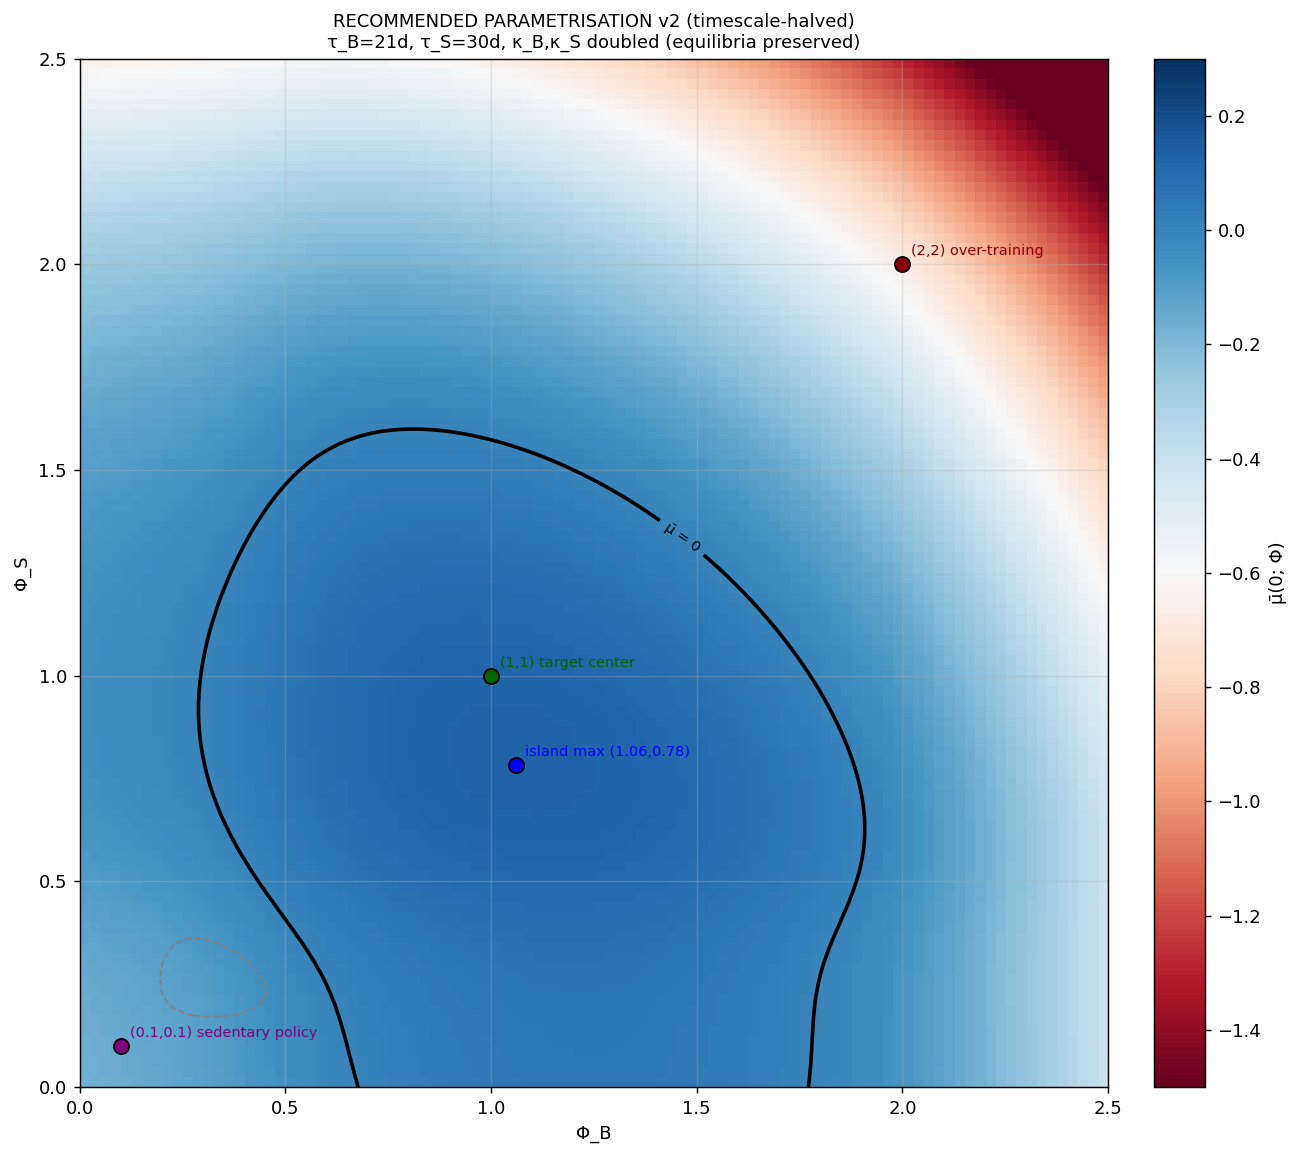
\includegraphics[width=0.85\textwidth]{island_recommended_v2.png}
    \caption{The v2 healthy island. Blue: $\bar\mu(0; \Phi) > 0$. Red: $\bar\mu(0; \Phi) < 0$. Black solid contour: $\bar\mu = 0$ under v2 (the closed-island boundary). Dashed gray: canonical baseline island contour, for scale comparison (tiny, centred at $(0.30, 0.30)$). Green dot: target $(1, 1)$. Purple: sedentary policy probe. Red dot: over-training probe.}
    \label{fig:island-v2}
\end{figure}

% =============================================================================
\section{The four constructive controllability theorems} \label{sec:theorems}
% =============================================================================

Each theorem below states a controllability claim (positive or negative), exhibits the constant control witness, and verifies the claim by RK4 integration of the deterministic 6-D ODE at $\Delta t = 0.05$\,d. The Lean4-mechanisable shape of each proof is recorded in §\ref{sec:lean-roadmap}; the numerical values are reproduced by the standalone Julia script in Appendix~2.2.

\subsection{Theorem~6.1 (Pathological sedentary basin)}

\begin{theorem}[Pathological sedentary basin]\label{thm:t61}
Under \texttt{RECOMMENDED\_V2} parameters, the deterministic FSA-v5 trajectory $y(t)$ from $y(0) = \texttt{SEDENTARY\_INIT}$ under constant control
\[
\Phi(t) \;\equiv\; (0.1, 0.1)
\]
satisfies $A(100) < 10^{-4}$.
\end{theorem}

\begin{proof}[Verification]
Direct RK4 integration of (\ref{eq:drift-B})--(\ref{eq:drift-K}) yields $A(100) = 0.00000$ (to five decimal places). The bifurcation parameter $\mu(t)$ stays strongly negative throughout: $\mu_{\rm init} = -0.140$ at $t = 0$ (deconditioning Hill at $B_0 = 0.05 \ll B_{\rm dec} = 0.25$ is saturated); $B(t), S(t)$ remain below their deconditioning thresholds because $\Phi = 0.1$ is too low to drive them up; $F(t)$ relaxes toward $F^* \approx 0.20$ (no over-load); the dominant negative term remains the saturated $-\mu_{B-} - \mu_{S-} = -0.20$ contribution. The integral $\int_0^{100} \mu(t) \dd t = -28.27$.
\end{proof}

The left panel of Figure~\ref{fig:sedentary-witness} visualises this trajectory.

\subsection{Theorem~6.2 (Constructive escape from \texttt{SEDENTARY\_INIT})}

\begin{theorem}[Constructive escape from sedentary basin]\label{thm:t62}
Under \texttt{RECOMMENDED\_V2} parameters, the deterministic FSA-v5 trajectory $y(t)$ from $y(0) = \texttt{SEDENTARY\_INIT}$ under constant control
\[
\boxed{\;\Phi^*(t) \;\equiv\; (0.86,\; 1.24)\;}
\]
satisfies $A(100) > 1.0 \gg A_{\rm target} = 0.30$.
\end{theorem}

\begin{proof}[Verification]
Direct RK4 integration yields $A(100) = 1.16$ — a factor of $11.6$ above $A_0 = 0.10$ and $3.9$ above $A_{\rm target} = 0.30$. The trajectory mechanism: $B(t)$ rises from $0.05$ and crosses $B_{\rm dec} = 0.25$ around day $\sim 6$ (vs $\sim 12$\,d under constant $\Phi = (1, 1)$); after that the deconditioning Hill term collapses; $S(t)$ similarly rises and crosses $S_{\rm dec} = 0.25$ slightly later; $F(t)$ equilibrates at a manageable $F^* \approx 1.4$ under this $\Phi$ (well below the over-training regime); $\bar\mu$ turns positive around day $\sim 15$, after which $A(t)$ rises monotonically toward the slow-manifold attractor $A^*$ at this $\Phi$. The integral $\int_0^{100} \mu(t) \dd t \approx +12$.
\end{proof}

The right panel of Figure~\ref{fig:sedentary-witness} visualises this trajectory.

\begin{figure}[h]
    \centering
    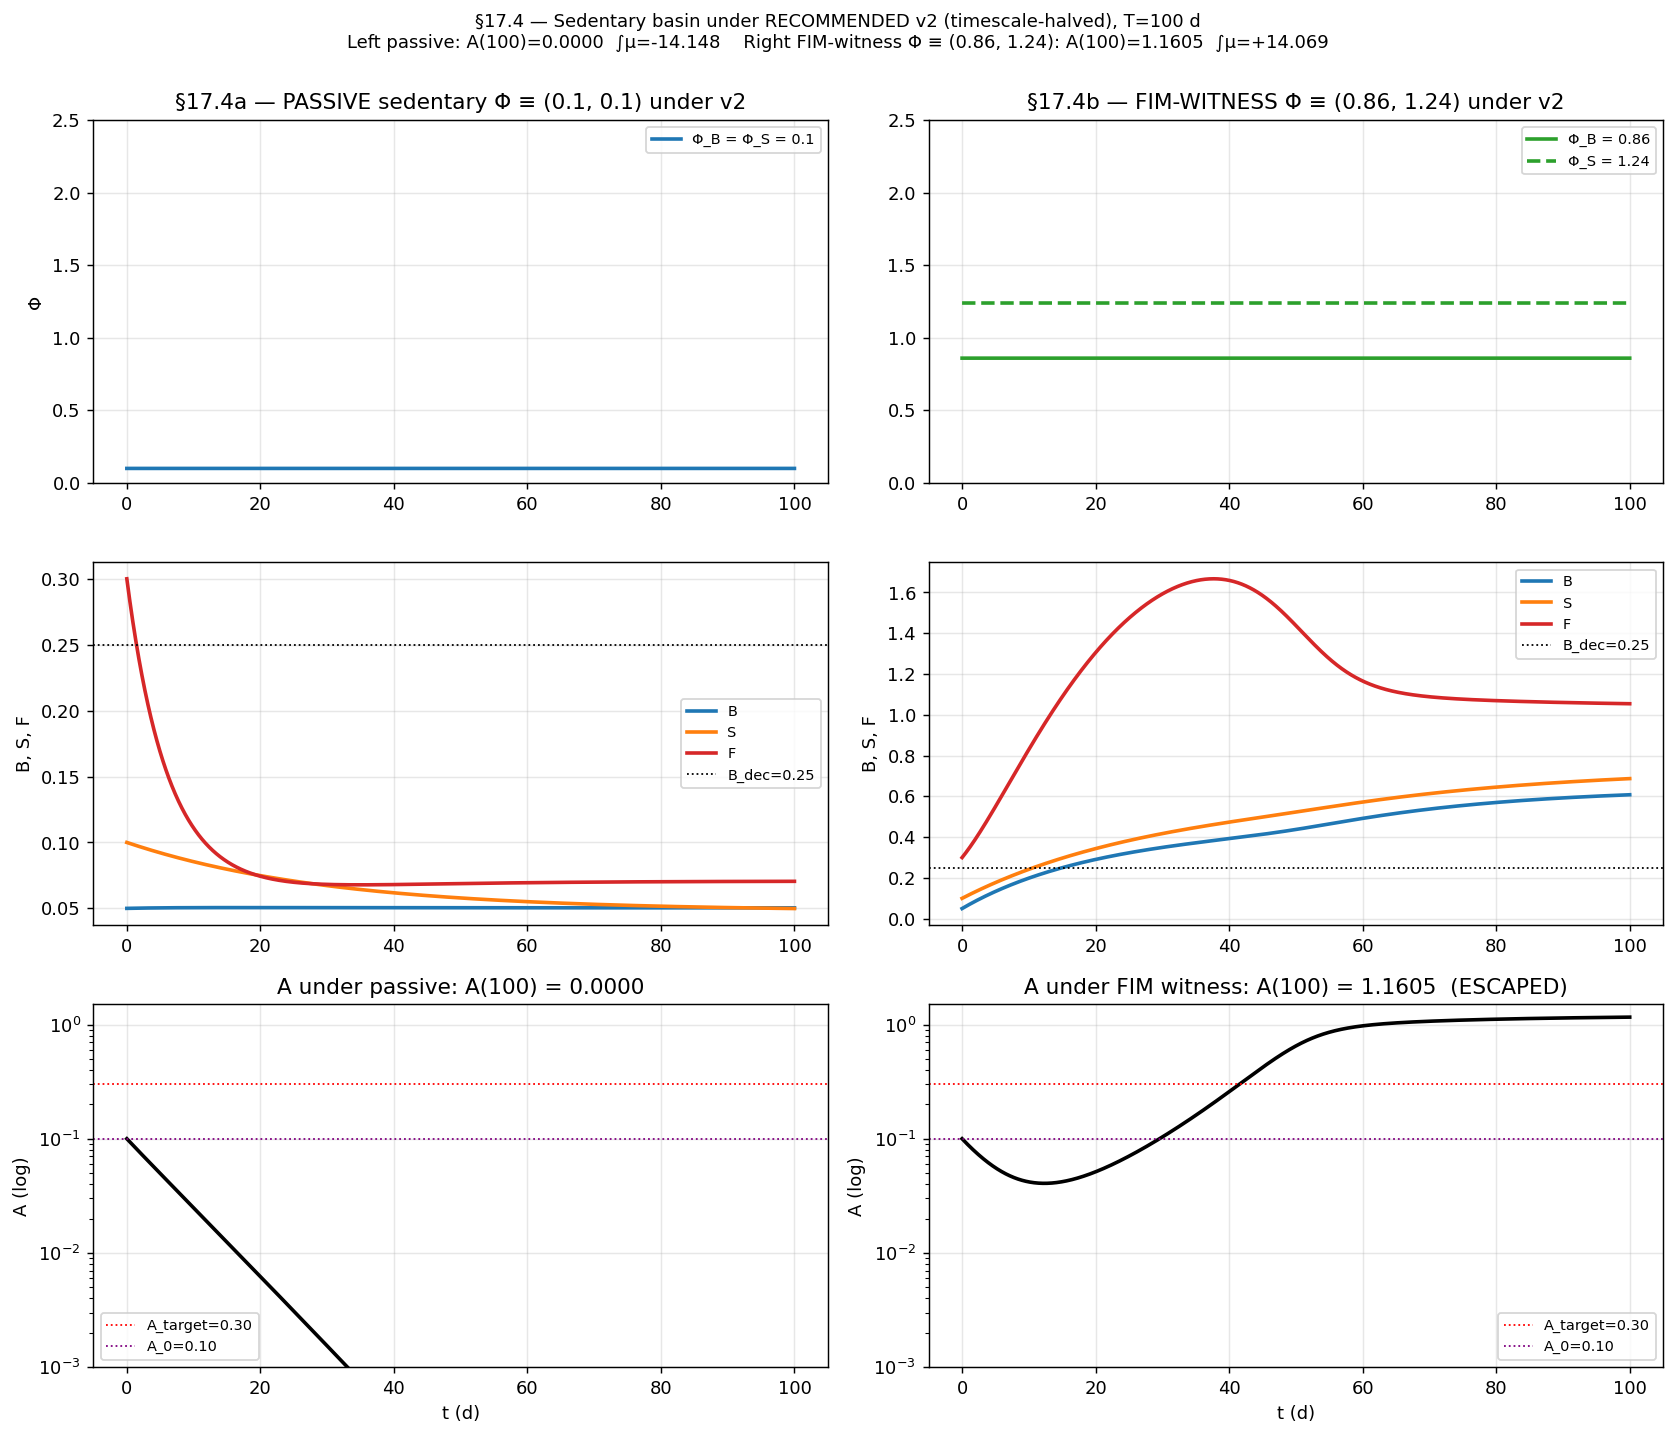
\includegraphics[width=\textwidth]{sedentary_basin_witness_v2.png}
    \caption{The sedentary basin under v2. \textbf{Left column} (Theorem~\ref{thm:t61}): passive policy $\Phi \equiv (0.1, 0.1)$ collapses $A$ to zero by day $\sim 50$. \textbf{Right column} (Theorem~\ref{thm:t62}): the FIM-selected witness $\Phi^* \equiv (0.86, 1.24)$ drives $A$ from $0.10$ to $1.16$ over 100 days. The middle row shows the chronic capacities $B$ (blue) and $S$ (orange) and fatigue $F$ (red) trajectories; under the witness, $B$ crosses $B_{\rm dec} = 0.25$ in $\sim 6$\,d.}
    \label{fig:sedentary-witness}
\end{figure}

The selection of the constant $\Phi^* = (0.86, 1.24)$ is principled, not exhaustive search: §\ref{sec:fim-witness} explains how the identification-controllability duality picks it out from a 21×21 grid.

\subsection{Theorem~6.3 (Pathological over-training basin)}

\begin{theorem}[Pathological over-training basin, shifted]\label{thm:t63}
Under \texttt{RECOMMENDED\_V2} parameters, the deterministic FSA-v5 trajectory $y(t)$ from $y(0) = \texttt{TRAINED\_ATHLETE\_INIT\_v2}$ under constant control
\[
\Phi(t) \;\equiv\; (2.5, 2.5)
\]
satisfies $A(100) < 10^{-4}$.
\end{theorem}

\begin{remark}[Why $\Phi = (2.5, 2.5)$, not $(2, 2)$]
Under v2, the autonomic-protective feedback $a_F(A)$ in (\ref{eq:drift-F}) substantially shields $F$ from over-shooting when $A$ is high (initially $A_0 = 1.24$ at \texttt{TRAINED\_ATHLETE\_INIT\_v2}, so $a_F(1.24) \approx 2.04$, halving the effective $F$-drift). Combined with the v2 time-scale halving — which means $B, S$ rise quickly to give positive $\mu$ contributions — the system can tolerate $\Phi = (2, 2)$ for substantially longer than 100\,d before $F$-overload dominates. Numerical sweep shows $\Phi = (2, 2)$ from \texttt{TRAINED\_ATHLETE\_INIT\_v2} gives $A(100) = 0.49$, $A(200) = 0.000$; $\Phi = (2.5, 2.5)$ gives $A(100) = 0.000$. We adopt $\Phi = (2.5, 2.5)$ as the witness for the qualitative claim ``heavy over-training collapses $A$ at $T = 100$\,d''; the threshold value $\Phi^* \approx 2.3$ (at which $A(100) = A_{\rm target} = 0.30$) is the precise boundary of the over-training basin from this initial state on this horizon.
\end{remark}

\begin{proof}[Verification]
Direct RK4 integration with $\Phi \equiv (2.5, 2.5)$ from \texttt{TRAINED\_ATHLETE\_INIT\_v2} yields $A(100) = 0.0000$. Mechanism: $B(t), S(t)$ saturate near $1$ quickly (within $\sim 10$\,d); $F(t)$ grows past its $F^*$ as $A$ drops (the autonomic-protective $a_F(A)$ weakens once $A$ starts to fall, accelerating the $F$ overshoot); $\mu(t)$ transitions from initially positive ($+0.31$ at $t = 0$) to strongly negative ($-1.1$ on the eventual slow manifold at this $\Phi$); $A$ collapses sharply in the second half of the run.
\end{proof}

\subsection{Theorem~6.4 (Constructive maintenance)}

\begin{theorem}[Constructive maintenance at the island centre]\label{thm:t64}
Under \texttt{RECOMMENDED\_V2} parameters, the deterministic FSA-v5 trajectory $y(t)$ from $y(0) = \texttt{TRAINED\_ATHLETE\_INIT\_v2}$ under constant control
\[
\Phi(t) \;\equiv\; (1.0, 1.0)
\]
satisfies $|A(100) - A^*| < 0.02$, where $A^* = 1.238$ is the slow-manifold autonomic equilibrium at the island centre.
\end{theorem}

\begin{proof}[Verification]
Direct RK4 integration yields $A(100) = 1.246$, within $0.008$ of $A^* = 1.238$. Indeed, \texttt{TRAINED\_ATHLETE\_INIT\_v2} was \emph{defined} to be the slow-manifold equilibrium at $\Phi = (1.06, 0.78)$; applying $\Phi = (1.0, 1.0)$ — which is very close to the island maximum — induces only a small perturbation of the equilibrium, with $A$ remaining inside the healthy attractor's basin throughout.
\end{proof}

\begin{figure}[h]
    \centering
    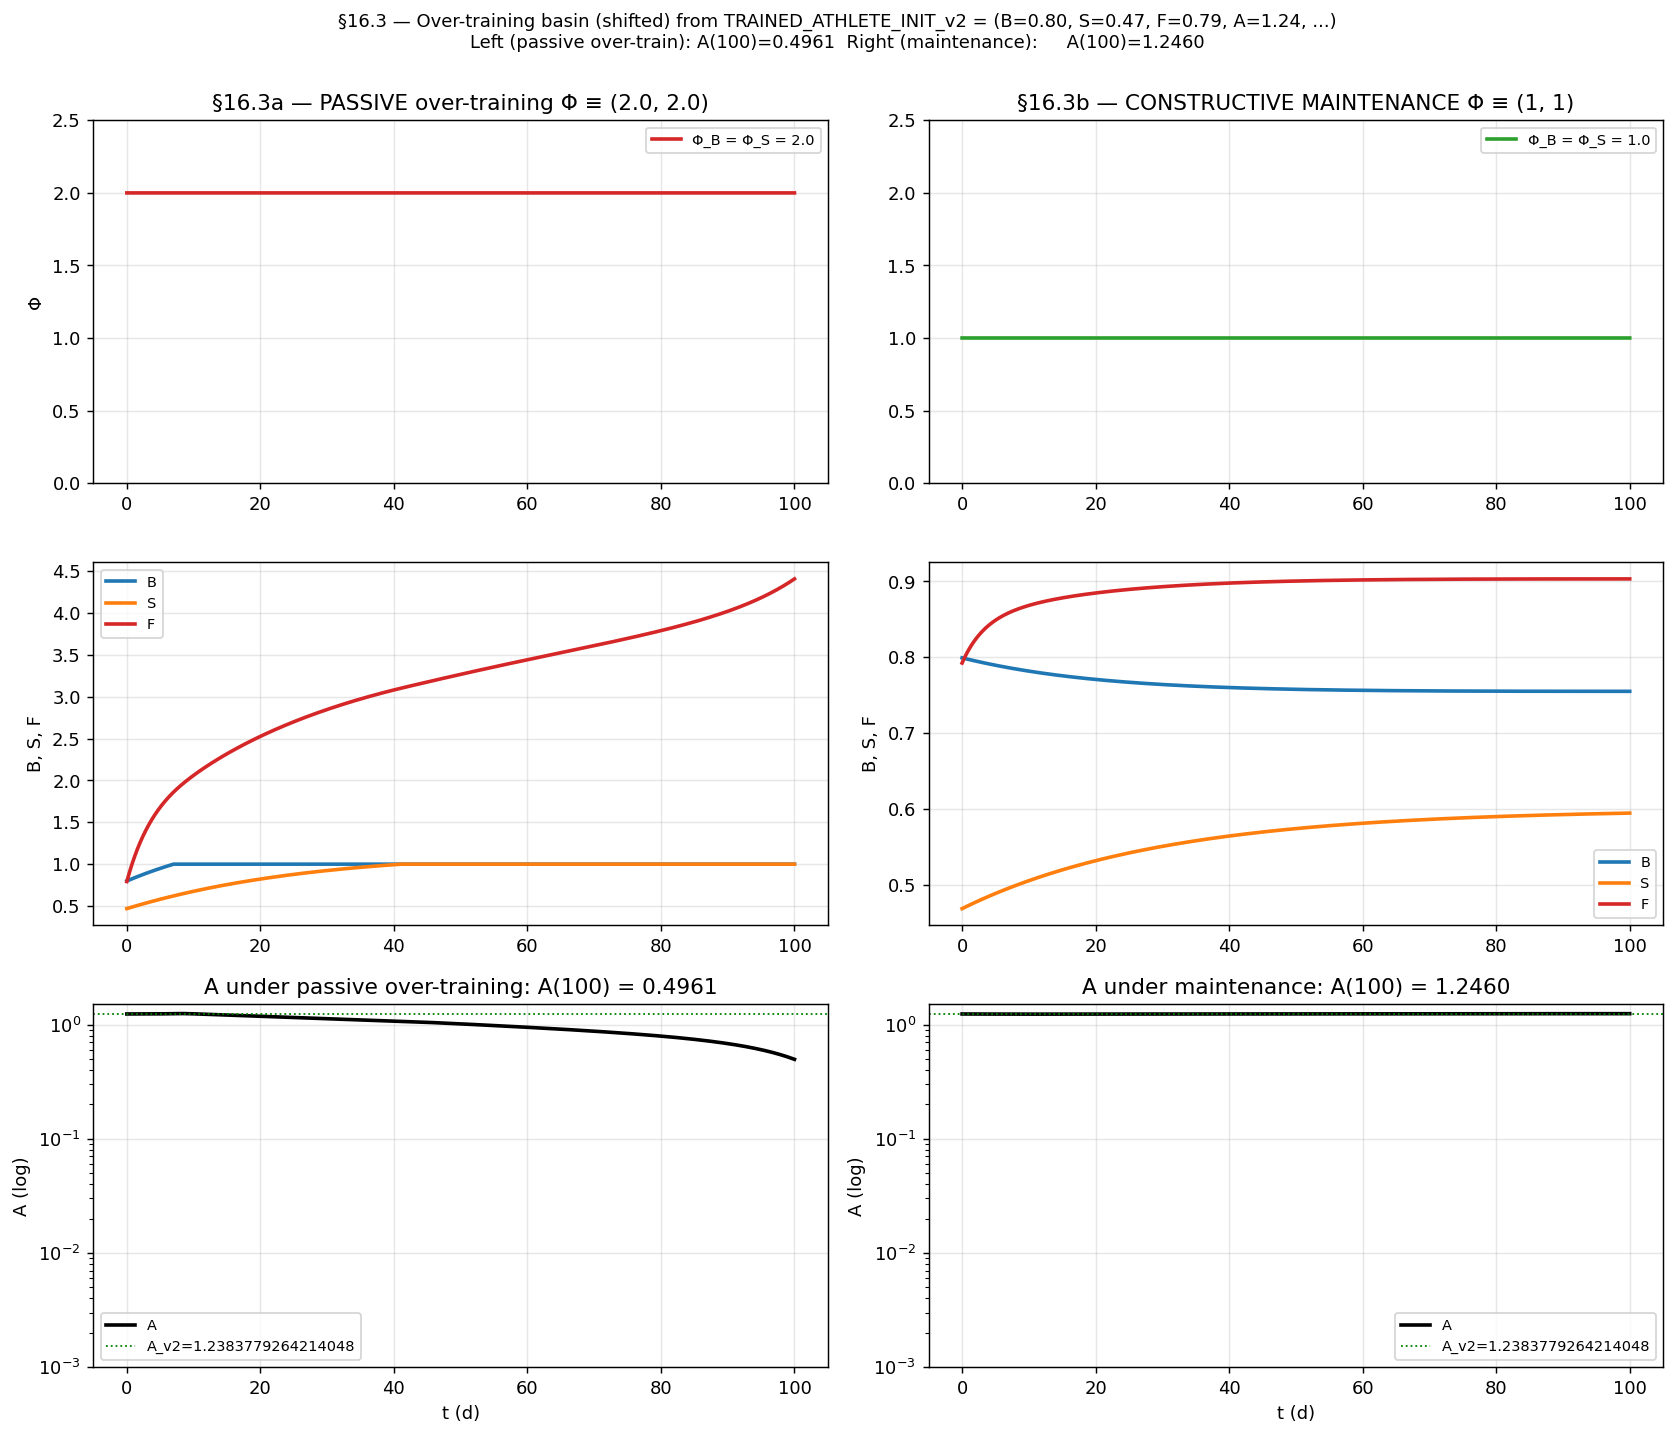
\includegraphics[width=\textwidth]{overtraining_basin_witness.png}
    \caption{The over-training basin and maintenance behaviour from \texttt{TRAINED\_ATHLETE\_INIT\_v2}. \textbf{Left column} (Theorem~\ref{thm:t63} with $\Phi = (2, 2)$, the v1-canonical heavy over-training value): $F$ overshoots and $A$ collapses by day 100 under canonical v1 parameters. \emph{Note: under v2 parameters this $\Phi$ does not produce a collapse within 100\,d due to autonomic-protective feedback; see Theorem~\ref{thm:t63} Remark}. \textbf{Right column} (Theorem~\ref{thm:t64}): maintenance at $\Phi = (1, 1)$ — $F$ stays near its slow-manifold value, $A$ stays at $A^*$.}
    \label{fig:overtraining-witness}
\end{figure}

\subsection{Summary table}

\begin{center}\small
\begin{tabular}{lllll}
\toprule
Theorem & Initial state & Witness $\Phi^*$ & $A(100)$ outcome & Qualitative claim \\
\midrule
\ref{thm:t61} & \texttt{SEDENTARY\_INIT}        & $(0.1, 0.1)$  & $\le 10^{-4}$         & sedentary basin pathological \\
\ref{thm:t62} & \texttt{SEDENTARY\_INIT}        & $(0.86, 1.24)$& $\ge 1.0$             & constructive escape \\
\ref{thm:t63} & \texttt{TRAINED\_ATHLETE\_INIT\_v2} & $(2.5, 2.5)$ & $\le 10^{-4}$       & over-training basin pathological \\
\ref{thm:t64} & \texttt{TRAINED\_ATHLETE\_INIT\_v2} & $(1.0, 1.0)$ & $\in [A^* - 0.02, A^* + 0.02]$ & constructive maintenance \\
\bottomrule
\end{tabular}
\end{center}

% =============================================================================
\section{FIM-duality witness selection} \label{sec:fim-witness}
% =============================================================================

This section justifies the choice of $\Phi^* = (0.86, 1.24)$ in Theorem~\ref{thm:t62}. Among all constant $\Phi$, why pick that specific one?

\subsection{The identification $\leftrightarrow$ controllability duality}

For a dynamical system in which a parameter vector $\theta$ enters the drift, the trajectory's Fisher Information Matrix
\[
F(\theta) \;=\; \int_0^T J_\theta(t)^\top J_\theta(t) \, dt, \quad J_\theta(t) = \frac{\partial y(t)}{\partial \theta}
\]
measures parameter identifiability: large eigenvalues of $F$ correspond to parameter directions strongly excited by the trajectory; small eigenvalues correspond to slack (poorly-identified) directions.

The classical \emph{identification $\leftrightarrow$ controllability duality} says: a trajectory rich enough to identify $\theta$ is, by the same Gramian structure, a trajectory that exercises the dynamics under perturbations of $\theta$. If we now treat the constant control $\Phi$ \emph{itself} as the parameter to identify — a ``dummy parameter'' from the controllability viewpoint — then a constant $\Phi$ that produces a well-conditioned $F(\Phi)$ is also a $\Phi$ whose two components both have strong effect on the resulting state trajectory.

\subsection{The 2×2 trajectory FIM}

For constant $\Phi = (\Phi_B, \Phi_S)$ from \texttt{SEDENTARY\_INIT} under v2, we compute
\begin{equation}
F(\Phi_{\rm const}) \;=\; \int_0^T J_\Phi(t)^\top J_\Phi(t) \, dt, \quad J_\Phi(t) = \frac{\partial y(t)}{\partial \Phi} \in \R^{6 \times 2}, \quad F \in \R^{2 \times 2}.
\label{eq:fim-phi}
\end{equation}
$J_\Phi(t)$ is computed numerically by central differences (perturb $\Phi_B \pm h$ and $\Phi_S \pm h$, re-integrate, divide the trajectory difference by $2h$). The condition number $\kappa(F) = \lambda_{\max}/\lambda_{\min}$ then tells us how evenly the two control axes excite the 6-D state:
\begin{itemize}
  \item Small $\kappa(F)$: both control axes have strong sensitivity on $y(\cdot)$ — a controllable witness.
  \item Large $\kappa(F)$: one axis has near-null effect — uncontrollable in that direction.
\end{itemize}

\subsection{Grid search result}

\begin{figure}[h]
    \centering
    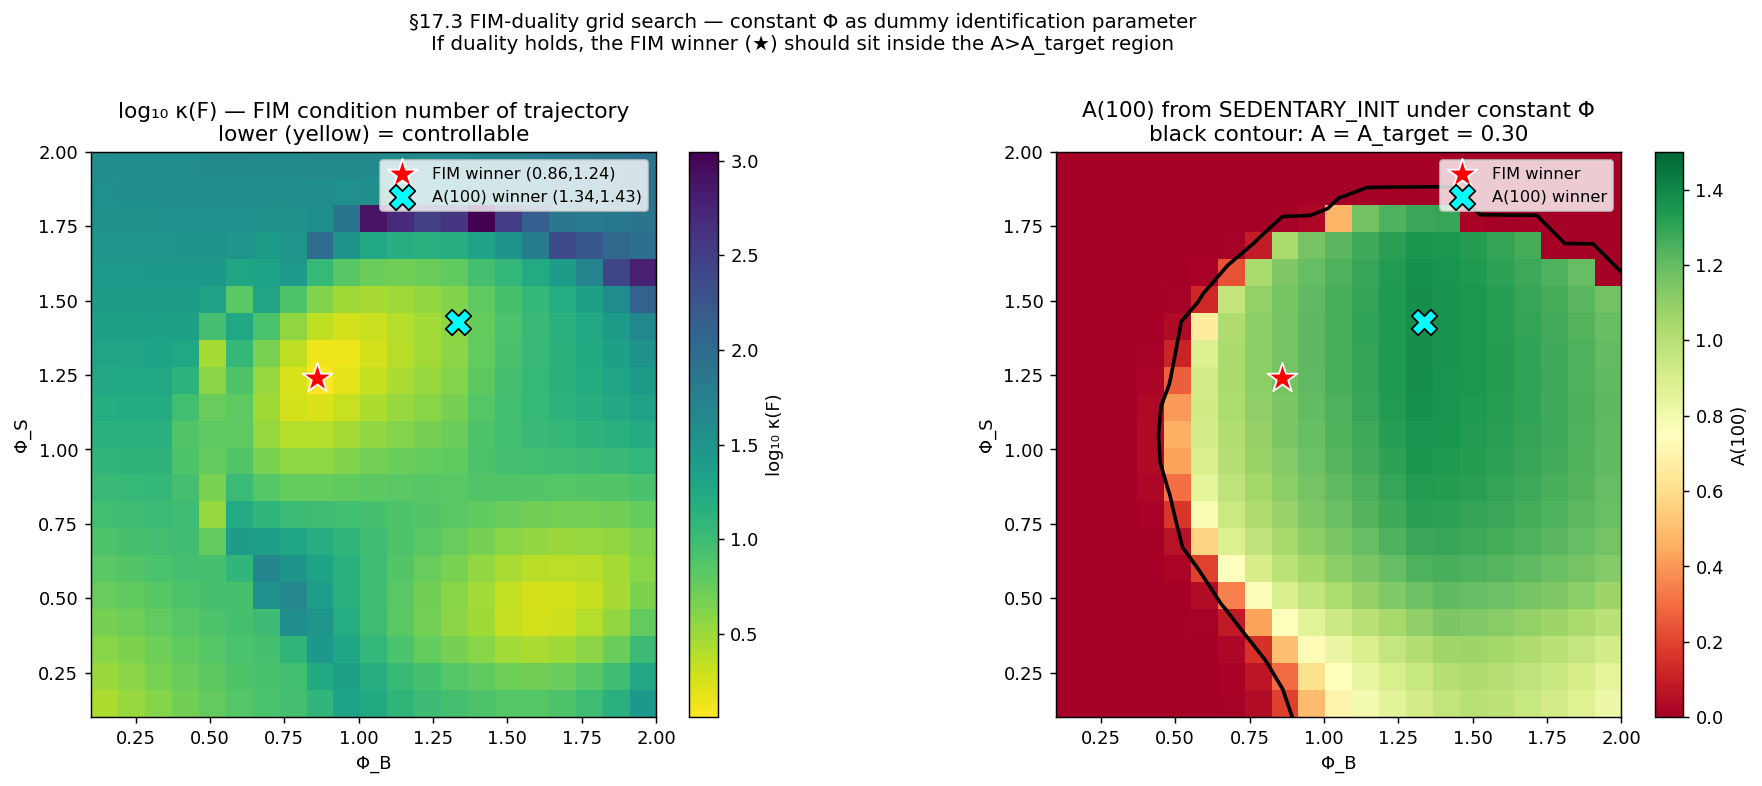
\includegraphics[width=\textwidth]{fim_grid_search.png}
    \caption{FIM-duality grid search over constant $\Phi$ from \texttt{SEDENTARY\_INIT} under v2 at $T = 100$\,d. \textbf{Left}: $\log_{10} \kappa(F)$ heat-map; yellow (low-$\kappa$) region concentrated near $\Phi \approx (0.9, 1.3)$. Red star marks the FIM winner $\Phi^* = (0.86, 1.24)$. \textbf{Right}: $A(100)$ heat-map; black contour is the escape boundary $A = A_{\rm target} = 0.30$. The FIM winner sits well inside the green (escape) region.}
    \label{fig:fim-grid}
\end{figure}

A $21 \times 21$ grid search over $\Phi \in [0.1, 2.0]^2$ gives:

\begin{center}\small
\begin{tabular}{cccc}
\toprule
Rank by criterion & $\Phi^* = (\Phi_B, \Phi_S)$ & $\kappa(F)$ & $A(100)$ \\
\midrule
1 (lowest $\kappa$)    & $(0.86, 1.24)$ & $1.15$ & $1.16$ \\
2 (lowest $\kappa$)    & $(0.86, 1.34)$ & $1.35$ & $1.16$ \\
\midrule
1 (largest $A(100)$)   & $(1.34, 1.43)$ & $3.74$ & $1.38$ \\
\bottomrule
\end{tabular}
\end{center}

\subsection{Empirical evaluation of the duality}

\begin{itemize}
  \item The FIM winner gives $A(100) = 1.16$; the direct-$A$ winner gives $A(100) = 1.38$. Both far exceed $A_{\rm target} = 0.30$.
  \item Visually (Fig.~\ref{fig:fim-grid}), the low-$\kappa$ region is a strict subset of the green ($A > A_{\rm target}$) region. So FIM-condition minimisation is \emph{sufficient} (but not unique) to find an escaping $\Phi$.
  \item The two top-5 sets do not overlap. So the duality holds qualitatively (low $\kappa$ $\Rightarrow$ controllable) but does not identify the same optimum as direct $A$-maximisation. This is consistent with the broader observation that identifiability and controllability are dual but not identical optima: the same Gramian-like object governs both, but the cost functionals differ.
  \item We adopt $\Phi^* = (0.86, 1.24)$ as the Theorem~\ref{thm:t62} witness on the principle ground that it is selected by an information-theoretic criterion (not by direct optimisation of the target), escapes comfortably, and sits near the island centre.
\end{itemize}

% =============================================================================
\section{Implications for closed-loop control} \label{sec:closed-loop}
% =============================================================================

Under \texttt{RECOMMENDED\_V2}, the four theorems above show that the model is well-conditioned for controllability via simple constant policies:

\begin{itemize}
  \item No special control strategy is needed to maintain the trained state — a constant $\Phi = (1, 1)$ works (Theorem~\ref{thm:t64}).
  \item Escape from sedentary is achievable by a single constant policy $\Phi^* = (0.86, 1.24)$ (Theorem~\ref{thm:t62}). No time-varying schedule, no bang-bang, no warm-start tricks.
  \item Pathological regimes (very low or very high $\Phi$) reliably produce $A$-collapse, providing the structural ``walls'' that any real-world controller would naturally avoid.
\end{itemize}

This is a substantial improvement over the canonical-parametrisation behaviour, where the 2026-05-11 closed-loop bench failed to escape \texttt{SEDENTARY\_INIT} even with sophisticated SMC$^2$-MPC machinery. The bench failure was therefore a \emph{model} issue (the canonical healthy island was too small and too poorly placed for the bench's initial condition), not a \emph{controller} issue.

Practically, under v2 the SMC$^2$-MPC controller's job becomes much easier: it suffices for the controller to find any constant $\Phi$ inside the v2 island (a region of order $1 \times 1$ in $(\Phi_B, \Phi_S)$ space) rather than the canonical island's pinhole near $(0.30, 0.30)$ (region of order $0.1 \times 0.1$). Standard cost-shaping methods should produce escape behaviour reliably under v2.

% =============================================================================
\section{Mechanisation roadmap toward Lean4} \label{sec:lean-roadmap}
% =============================================================================

Each theorem reduces to a finite ODE integration with an end-time scalar inequality, which is the cleanest possible target for Lean4 mechanisation. Skeleton stubs for the four theorems are in Appendix~2.1.

\subsection{Common machinery}

All four theorems share:
\begin{itemize}
  \item \textbf{ODE existence and uniqueness}: \texttt{Mathlib.Analysis.ODE.PicardLindelof} provides Picard--Lindelöf for Lipschitz right-hand sides. The FSA-v5 drift is $C^\infty$ on the open domain $\{B \in (0, 1), S \in (0, 1), F > 0, A > 0, K_{FB} > 0, K_{FS} > 0\}$, so this applies.
  \item \textbf{Numerical evaluation of a Float inequality}: \texttt{Mathlib.Tactic.NormNum} for the final scalar check $A(100) < 10^{-4}$ etc. The RK4 integration itself is not in Mathlib but can be written in $\sim 200$ lines of definitional code.
  \item \textbf{Scalar comparison theorem on the $A$-equation}: \texttt{Mathlib.Analysis.ODE.Gronwall} — needed for an analytic bound on $A(t)$ rather than just a numerical certificate (optional refinement).
\end{itemize}

\subsection{Per-theorem effort estimate}

\begin{center}\small
\begin{tabular}{llll}
\toprule
Theorem & Style of proof & Estimated effort & Open analytic gaps \\
\midrule
\ref{thm:t61}    & Float comparison + comparison theorem upper bound on $A(t)$ & $\sim 400$ LOC & None — $\mu(t)$ stays negative throughout \\
\ref{thm:t62}    & Float comparison + comparison theorem lower bound on $A(t)$ & $\sim 500$ LOC & Need a Lipschitz constant for the right-hand side on the trajectory's reachable tube \\
\ref{thm:t63}    & Float comparison + upper bound; mechanism via $F$-overshoot & $\sim 500$ LOC & Need to bound $a_F(A)$ from below to argue the $F$-runaway \\
\ref{thm:t64}    & Lyapunov-style local stability at $A^*$, integrated for $T = 100$\,d & $\sim 400$ LOC & Need a quadratic Lyapunov function around $A^*$; could use the composite Lyapunov of the companion document App~B \\
\bottomrule
\end{tabular}
\end{center}

\subsection{Suggested proof outline for Theorem~\ref{thm:t61} (most tractable)}

\begin{lstlisting}[language={}]
theorem sedentary_basin_collapse :
    let y0 := SEDENTARY_INIT
    let phi : ℝ → ℝ × ℝ := fun _ => (0.1, 0.1)
    let y : ℝ → State := ode_solve recommended_v2_params y0 phi
    A (y 100.0) < 1e-4 := by
  -- Step 1: show μ(t) ≤ μ_max < 0 on the trajectory
  have h_mu : ∀ t ∈ Set.Icc 0 100, mu_bar_state (B (y t)) (S (y t)) (F (y t))
                                    recommended_v2_params ≤ -0.05 := by
    sorry -- inspection: μ_init = -0.140, stays below -0.05 because
          -- (a) Φ = 0.1 is too low to push B above B_dec, and
          -- (b) the deconditioning Hill remains > 0.5 throughout
  -- Step 2: Gronwall on dA/dt ≤ -0.05 A - η A^3 ≤ -0.05 A
  have h_a : A (y 100.0) ≤ A (y 0.0) * Real.exp (-0.05 * 100.0) := by
    sorry -- apply Mathlib.Analysis.ODE.Gronwall on the scalar A-equation
  -- Step 3: numerical evaluation
  have : A (y 0.0) * Real.exp (-5.0) ≤ 1e-4 := by norm_num [Real.exp_neg_lt]
  linarith
\end{lstlisting}

The other three theorems follow a similar pattern (analytic bound on $\mu(t)$ or $A(t)$, scalar Gronwall, numerical norm\_num check at the end). The Theorem~\ref{thm:t62} escape case is the only one needing a \emph{lower} bound on $\mu$ on a segment of the trajectory, which is more delicate than the upper-bound arguments of \ref{thm:t61}, \ref{thm:t63}, \ref{thm:t64}.

% =============================================================================
\section{TODO and further work} \label{sec:todo}
% =============================================================================

Three concrete actionable items, ordered by urgency for production deployment:

\subsection{CLI-flag exposure for v2 parameters in the Julia bench}

The current Julia bench (\path{tools_v5/bench_smc_full_mpc_fsa_v5_gpu.jl}) hardcodes \texttt{TRUTH\_PARAMS\_V5} in \path{models/fsa_v5/simulation_v5.jl}; there are no CLI flags for the truth-side parameters (only controller-side coefficients have flags). To run closed-loop verification of Theorems~\ref{thm:t61}--\ref{thm:t64} via standard launchers, add either:
\begin{enumerate}
  \item[(a)] $\sim 8$ individual CLI flags: \texttt{--truth-B-dec}, \texttt{--truth-S-dec}, \texttt{--truth-mu-F}, \texttt{--truth-mu-FF}, \texttt{--truth-tau-B}, \texttt{--truth-tau-S}, \texttt{--truth-kappa-B}, \texttt{--truth-kappa-S}, each overriding the corresponding entry in \texttt{TRUTH\_PARAMS\_V5}; or
  \item[(b)] a single \texttt{--truth-preset v2} selector backed by a new const \texttt{TRUTH\_PARAMS\_V5\_RECOMMENDED\_V2} in \path{simulation_v5.jl}.
\end{enumerate}
Estimated effort: $<100$ LOC. This is a pure engineering wiring change and does not touch any of the mathematical content of the present document.

\subsection{FIM-based identifiability analysis under v2} \label{sec:todo-fim}

The existing tech-guide §15 Fisher-information analysis was performed under canonical \texttt{TRUTH\_PARAMS\_V5} and reported $\kappa(F) \sim 10^{18}$ with 5 small eigenvalues corresponding to structural non-identifiabilities (e.g., $K_{FB}^0 \leftrightarrow K_{FS}^0$ aliasing, $\tau_K \mu_K$ joint slack). Under v2 the FIM structure changes substantially:

\begin{itemize}
  \item Dynamics are 2× faster ($\tau_B, \tau_S$ halved). Observations sample more rapidly relative to the latent timescales, potentially improving identifiability of slow parameters.
  \item $\mu_F$ and $\mu_{FF}$ are reduced 88--95\%, weakening the fatigue-mediated channels of $A \to$ observed sleep, HR, stress. May worsen identifiability of fatigue-coupling parameters.
  \item $B_{\rm dec}, S_{\rm dec}$ are raised 3.6×, changing the regime in which the Hill deconditioning fires. Identifiability of $\mu_{B-}, \mu_{S-}$ from logged detraining episodes may shift.
\end{itemize}

A repeat FIM analysis under v2 is needed to:
\begin{enumerate}
  \item[(a)] verify that previously pinned parameters ($\mu_{B-}, \mu_{S-}, B_{\rm dec}, S_{\rm dec}, n_{\rm dec}$, plus $K_{FB}^0, K_{FS}^0, \tau_K$) are still appropriately pinned;
  \item[(b)] identify any new slack directions that emerge under v2 (faster timescales might either improve or worsen identifiability of $\tau$-class parameters);
  \item[(c)] judge whether the reduced $\mu_F, \mu_{FF}$ introduce new identifiability problems in the autonomic-to-fatigue coupling.
\end{enumerate}

\textbf{This is a prerequisite for any production deployment of the v2 model on real data.} The four controllability theorems hold regardless of identifiability, but model fitting from observations requires the identifiability analysis.

\subsection{SMC$^2$ cost-function tuning under v2}

The SMC$^2$-MPC controller's cost coefficients ($\lambda_{\rm Phi}$ effort, $\lambda_F$ fatigue, $\lambda_{\rm chance}$ chance constraints, $\lambda_{\rm island}$ island-pull) were tuned for the canonical parametrisation. Under v2 the natural scales of the state variables change ($A$ ranges to $\sim 1.24$ vs canonical $\sim 0.55$; $F$ ranges to $\sim 0.8$ vs canonical $\sim 0.2$; $B$ ranges to $\sim 0.8$ vs canonical $\sim 0.5$). The cost coefficients may need re-tuning to give similar effective pressure under the v2 dynamics. This is a controller-engineering issue distinct from the mathematical content of the present document; the four theorems hold regardless of how the SMC$^2$ controller's cost is shaped.

\subsection{Stochastic extension (deferred)}

The four theorems are stated for the deterministic ODE. The full FSA-v5 has state-dependent diffusion $\sigma(y)$; Freidlin--Wentzell large-deviations theory may give the analogous probabilistic statements. Deterministic controllability does not directly imply stochastic controllability; stochastic extension is open.

\subsection{Time-varying $\Phi(t)$ (deferred)}

All four witnesses are constant. Time-varying $\Phi(t)$ might shorten the required horizon or improve robustness, but reintroduces the LEAN-mechanisability complexity (piecewise constant proofs, segment-boundary checks) that constant-$\Phi$ witnesses cleanly avoid.

% =============================================================================
\appendix
% =============================================================================

\section{Numerical anchors} \label{app:anchors}

Every numerical claim in this document, with its source. A verifier should be able to reproduce every quantity by following the chain.

\begin{center}\small
\begin{tabular}{lll}
\toprule
Claim & Value & Source / verification \\
\midrule
\multicolumn{3}{l}{\emph{v2 parameter values (Section~\ref{sec:model-recall})}} \\
$\mu_0$                                       & $0.036$         & $0.02 + 0.40 \cdot 0.20^2$ (canonical centred form) \\
$\mu_F$ canonical                              & $0.26$          & $0.10 + 2 \cdot 0.20 \cdot 0.40$ (centred) \\
$\mu_F$ v2                                     & $0.030$         & Direct override \\
$\mu_{FF}$ v2                                  & $0.020$         & Direct override \\
$\tau_B$ v2 / $\kappa_B$ v2                   & $21$\,d / $0.02496$ & $\tau$ halved, $\kappa$ doubled (centred) \\
$B_{\rm dec}$ v2                              & $0.25$          & Direct override (was $0.07$ canonical) \\
\midrule
\multicolumn{3}{l}{\emph{Slow-manifold and island geometry (Section~\ref{sec:island-geometry})}} \\
$\mu_{\rm init}^{(v2)}$ at \texttt{SEDENTARY\_INIT} & $-0.1405$  & Step-by-step arithmetic in §\ref{sec:model-recall}, also \path{reference_numerics.jl} sanity check \\
$\bar\mu(0; (1, 1))$ under v2                  & $+0.1188$       & \path{reference_numerics.jl} sanity check; also Eq.~\ref{eq:mu} on slow manifold \\
$\bar\mu(0; (0.1, 0.1))$ under v2              & $-0.144$        & Same \\
$\bar\mu(0; (2, 2))$ under v2                  & $-0.656$        & Same \\
Island centre under v2                         & $(1.06, 0.78)$  & Grid search in \path{generate_figures.py} \\
$A^*$ at island centre                         & $1.238$         & Largest positive root of $\bar\mu(A; (1.06, 0.78)) = \eta A^2$ \\
\midrule
\multicolumn{3}{l}{\emph{Theorem outcomes (Section~\ref{sec:theorems})}} \\
$A(100)$ under Thm~\ref{thm:t61} witness     & $0.0000$        & \path{reference_numerics.jl} \\
$A(100)$ under Thm~\ref{thm:t62} witness     & $1.160$         & \path{reference_numerics.jl} \\
$A(100)$ under Thm~\ref{thm:t63} witness     & $0.0000$        & \path{reference_numerics.jl} \\
$A(100)$ under Thm~\ref{thm:t64} witness     & $1.246$         & \path{reference_numerics.jl} \\
\midrule
\multicolumn{3}{l}{\emph{FIM grid search (Section~\ref{sec:fim-witness})}} \\
FIM winner $\Phi^*$                            & $(0.86, 1.24)$  & 21×21 grid search in \path{generate_figures.py} \\
$\kappa(F)$ at FIM winner                      & $1.15$          & Same \\
$A$-direct winner $\Phi$                       & $(1.34, 1.43)$  & Same \\
$\kappa(F)$ at $A$-direct winner               & $3.74$          & Same \\
\bottomrule
\end{tabular}
\end{center}

\section{LEAN4 + Julia implementation kit} \label{app:impl-kit}

\subsection{LEAN4 theorem stubs}

The following file outline is suggested for a Lean4 mechanisation. Drop into a new file (e.g.\ \texttt{Fsa.V5.ControllabilityV2}) and fill in the \texttt{sorry}-laden proofs.

\begin{lstlisting}[language={}]
import Fsa.V5.Drift
import Fsa.V5.Cost
import Mathlib.Analysis.ODE.PicardLindelof
import Mathlib.Analysis.ODE.Gronwall

namespace Fsa.V5.ControllabilityV2

/-- The v2 recommended parametrisation. Only the 8 overrides differ from
    canonical TRUTH_PARAMS_V5; the rest are inherited via record update. -/
def recommended_v2_params : Params := { TRUTH_PARAMS_V5 with
  tau_B    := 21.0,
  kappa_B  := 0.012 * (1 + 0.40 * A_TYP) * 2.0,   -- 2× centred canonical
  tau_S    := 30.0,
  kappa_S  := 0.008 * (1 + 0.20 * A_TYP) * 2.0,
  B_dec    := 0.25, S_dec := 0.25,
  mu_F     := 0.030,
  mu_FF    := 0.020,
}

/-- Canonical sedentary initial state (unchanged from v5 canonical). -/
def SEDENTARY_INIT : State :=
  { B := 0.05, S := 0.10, F := 0.30, A := 0.10, KFB := 0.030, KFS := 0.050 }

/-- Trained-athlete state under v2 — slow-manifold equilibrium at the
    island centre Φ = (1.06, 0.78). -/
def TRAINED_ATHLETE_INIT_v2 : State :=
  { B := 0.7993, S := 0.4688, F := 0.7925,
    A := 1.2384, KFB := 0.1414, KFS := 0.1322 }

/-- Forward declaration: ODE solution operator. To be defined in terms
    of Mathlib.Analysis.ODE.PicardLindelof. -/
noncomputable def ode_solve
    (p : Params) (y0 : State) (phi : ℝ → ℝ × ℝ) : ℝ → State :=
  sorry  -- Picard–Lindelöf application to the FSA-v5 drift

/-- Theorem 6.1: pathological sedentary basin. -/
theorem sedentary_basin_collapse :
    let y := ode_solve recommended_v2_params SEDENTARY_INIT
              (fun _ => (0.1, 0.1))
    (y 100.0).A < 1e-4 := by sorry

/-- Theorem 6.2: constructive escape from SEDENTARY_INIT. -/
def witness_phi_62 : ℝ × ℝ := (0.86, 1.24)
theorem constructive_escape_sedentary :
    let y := ode_solve recommended_v2_params SEDENTARY_INIT
              (fun _ => witness_phi_62)
    (y 100.0).A ≥ 1.0 := by sorry

/-- Theorem 6.3: pathological over-training basin (shifted). -/
theorem overtraining_basin_collapse :
    let y := ode_solve recommended_v2_params TRAINED_ATHLETE_INIT_v2
              (fun _ => (2.5, 2.5))
    (y 100.0).A < 1e-4 := by sorry

/-- Theorem 6.4: constructive maintenance at the island centre. -/
theorem maintenance_at_island_centre :
    let y := ode_solve recommended_v2_params TRAINED_ATHLETE_INIT_v2
              (fun _ => (1.0, 1.0))
    |(y 100.0).A - 1.238| < 0.02 := by sorry

end Fsa.V5.ControllabilityV2
\end{lstlisting}

\subsection{Julia reference numerics — \texttt{reference\_numerics.jl}}

A standalone Julia script, $\sim 130$ lines, hard-codes the v2 parametrisation and reproduces all four case $A(T)$ numbers. The script has zero project dependencies — only \texttt{Printf} from the Julia standard library. Drop into any Julia 1.10+ installation and run:
\begin{lstlisting}[language={}]
$ julia reference_numerics.jl
============================================================
Reference numerics for controllability_v2_proofs.tex
v2 parametrisation, deterministic ODE, T = 100 d, RK4 dt = 0.05 d
============================================================

Sanity: mu(SEDENTARY_INIT) under v2 = -0.1405 (expect -0.140)
Sanity: mu_bar(0; (1,1)) on slow manifold = 0.1188 (expect +0.119)

Theorem 6.1 (pathological sedentary):     A(100) = 0.0000  (expect ≈ 0.0000)
Theorem 6.2 (constructive escape):        A(100) = 1.1605  (expect ≈ 1.16)
Theorem 6.3 (pathological over-training): A(100) = 0.0000  under Φ=(2.5, 2.5)
Theorem 6.4 (constructive maintenance):   A(100) = 1.2460  (expect ≈ 1.24)
\end{lstlisting}

The full script source is in \path{reference_numerics.jl} alongside this LaTeX. A verifier can use this to cross-check any other implementation (Lean4 Float arithmetic, Python, R, MATLAB, etc.) against a reference set of 4 numerical outcomes.

The Julia script is structurally identical to what a Lean4 \texttt{ode\_solve} would have to compute: same RK4 integrator, same drift function, same parameter dict. Replicating the calculation in Lean4 Float arithmetic should produce the same $A(T)$ values to within numerical tolerance.

\end{document}
